\chapter{质量守恒与配平的方程式}\label{ch:g8:balanced-equations}

一根重两千克的木柴在壁炉中\omterm{def:g4:what-a-fire-needs:burning}{燃烧}。早晨，
只剩下几十克灰白色的灰烬。将近两千克的物质
难道就在夜里消失了吗？几个世纪以来无人能说清。答案来自一位化学家，
他决定把一切都称一称——
包括没有人想过要称量的气体。

\begin{recall}
在\omterm{def:g7:chemical-reactions:reaction}{化学反应}中，\omterm{def:g7:chemical-reactions:reactant}{反应物}被消耗，生成物被生成；
\omterm{def:g7:chemical-reactions:reactant}{反应物}的\omterm{def:g7:atoms-and-molecules:atom}{原子}重新排列成生成物，
\omterm{def:g7:atoms-and-molecules:atom}{原子}既不会被创造，也不会消失（见\cref{ch:g7:chemical-reactions}）。
化学式如 \ce{H2O} 列出一个\omterm{def:g7:atoms-and-molecules:molecule}{分子}中的\omterm{def:g7:atoms-and-molecules:atom}{原子}；写在前面的
数字，如 \ce{3H2O}，表示\omterm{def:g7:atoms-and-molecules:molecule}{分子}的个数，
即（见\cref{ch:g7:atoms-and-molecules}）。
\end{recall}

\begin{omfigure}
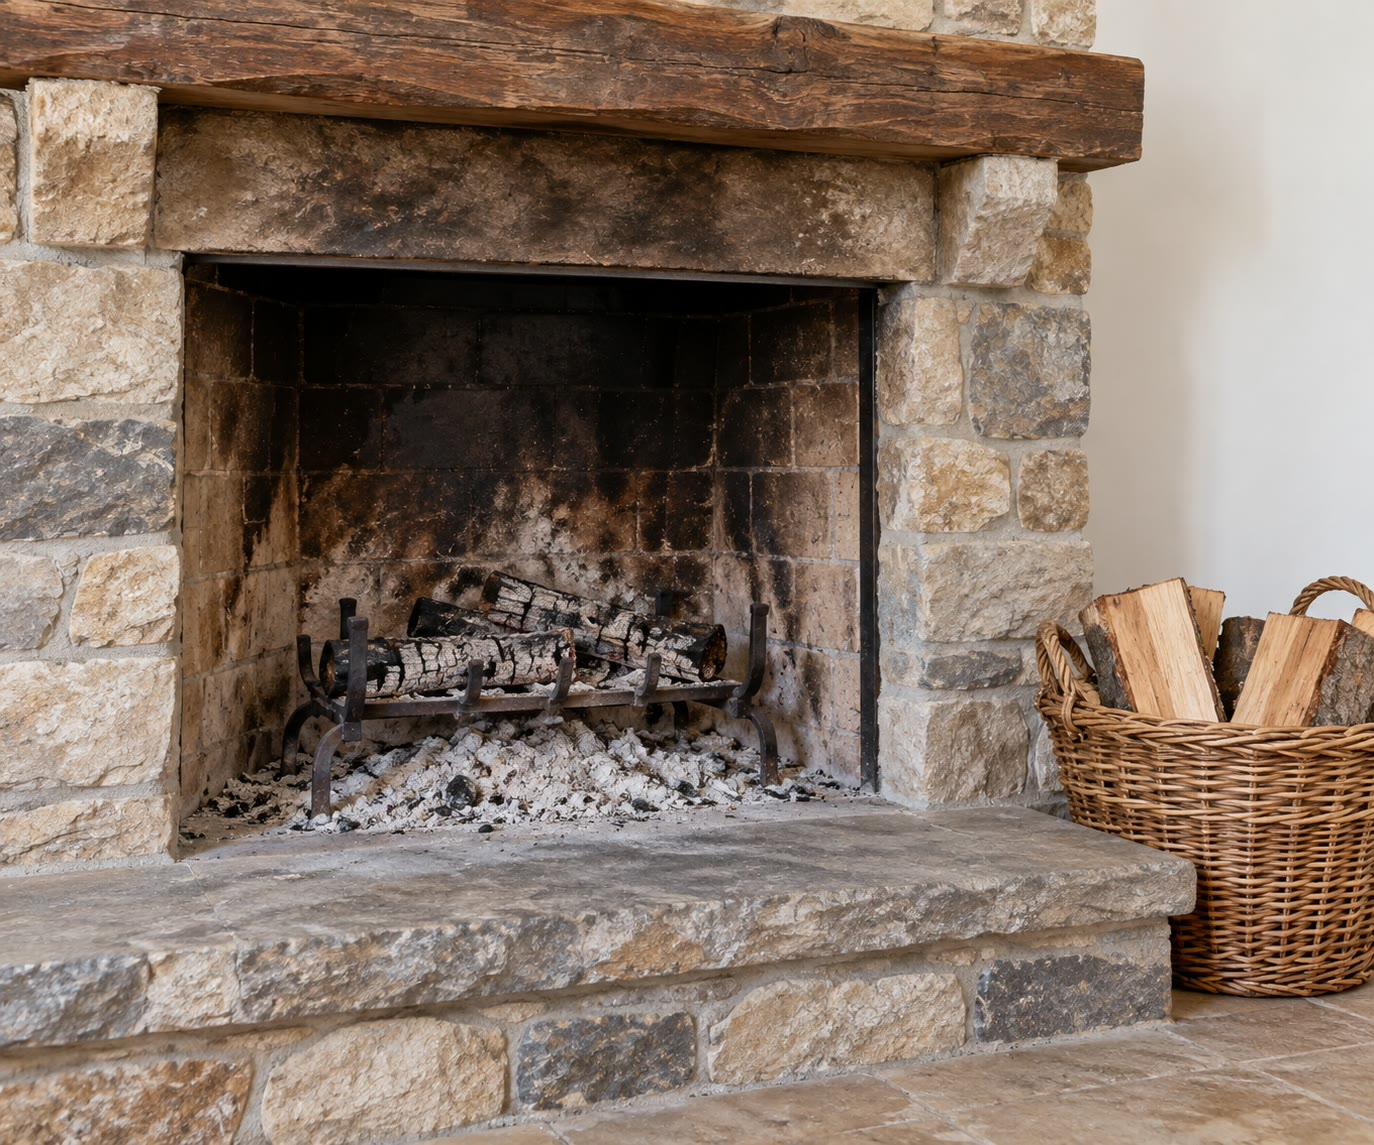
\includegraphics[width=0.5\linewidth]{images/book1/ai/g8-fireplace-ash.jpg}

{\small 次日早晨的壁炉：木柴烧后只剩下
少量灰烬。}
\end{omfigure}

\section{质量是守恒的}

\begin{inthelab}[在密闭锥形瓶中称量反应]
老师在锥形瓶中加入一些醋，把小苏打放入气球中，
气球套在瓶口，然后将整套装置放在天平上：\qty{212.4}{g}。
将气球提起，使小苏打落入醋中：
\omterm{def:g6:pure-substances-and-mixtures:mixture}{混合物}冒泡，气球因生成的气体而鼓起。天平
示数仍为 \qty{212.4}{g}。同样的反应若在敞口锥形瓶中进行，不用气球，
则质量“减少”了：气体逸散到房间里。
\end{inthelab}

\begin{omfigure}
\begin{tikzpicture}[font=\small, scale=1.15]
  % closed flask
  \pic[transform shape] at (0,0) {balance};
  \pic[transform shape] at (0,0.8) {erlenmeyer={0.25}{omWater!80}};
  \fill[red!55, draw=red!60!black] (0,4.05) ellipse (0.5 and 0.62);
  \fill[red!55] (-0.3,3.45) rectangle (0.3,3.6);
  \node[anchor=north, align=center] at (0,-0.1) {密闭：气体留在 \\气球中};
  \node[anchor=west, font=\footnotesize] at (1.25,0.3) {\qty{212.4}{g}};
  % open flask
  \pic[transform shape] at (4,0) {balance};
  \pic[transform shape] at (4,0.8) {erlenmeyer={0.25}{omWater!80}};
  \foreach \y in {3.6,3.95,4.3} \draw[->, black!45, decorate,
    decoration={snake, amplitude=0.6pt, segment length=4pt}] (4,\y) -- (4,\y+0.3);
  \node[anchor=north, align=center] at (4,-0.1) {敞口：气体逸出，\\示数下降};
  \node[anchor=west, font=\footnotesize] at (5.25,0.3) {\qty{211.9}{g}};
\end{tikzpicture}

{\small 同一反应的称量结果。密闭锥形瓶中，质量
不变；敞口锥形瓶中，气体逸出，天平示数
变小。}
\end{omfigure}

\begin{definition}[质量守恒]\label{def:g8:balanced-equations:conservation}
\emph{质量守恒}\index{质量守恒}是这样一条定律：
在\omterm{def:g7:chemical-reactions:reaction}{化学反应}中，生成物的总质量
等于参加反应的\omterm{def:g7:chemical-reactions:reactant}{反应物}的总质量。
既无损失，也无产生；物质只是改变了形态。
\end{definition}

\begin{example}[认真称量的木柴]\label{ex:g8:balanced-equations:log}
若能在\omterm{def:g4:what-a-fire-needs:burning}{燃烧}前称量\omterm{def:g4:what-a-fire-needs:burning}{燃烧}的木柴以及它从\omterm{def:g4:air-a-mixture-of-gases:air}{空气}中夺取的氧气，
并在\omterm{def:g4:what-a-fire-needs:burning}{燃烧}后称量灰烬、二氧化碳和水蒸气，则两者的总质量
应当相等。灰烬很轻，是因为大部分生成物
是随烟囱排出的气体。
\end{example}

\begin{history}[拉瓦锡称量一切，1770 年代--1789 年]
安托万-洛朗·拉瓦锡立下了一条规矩：
每次反应前后都称量每种物质，并在密封容器中进行，
使气体既不能逸出，也不能进入。他证明了金属
生锈或\omterm{def:g4:what-a-fire-needs:burning}{燃烧}时质量增加，是因为从\omterm{def:g4:air-a-mixture-of-gases:air}{空气}中夺取了某种物质——氧气，
这种气体是他命名的；他于 1789 年指出，\omterm{def:g7:chemical-reactions:reaction}{化学反应}中既不会有物质被创造，
也不会消失。他的妻子玛丽-安娜·保尔兹·拉瓦锡与他并肩工作，
记录实验，并为他的著作绘制仪器图。
\end{history}

\begin{omfigure}
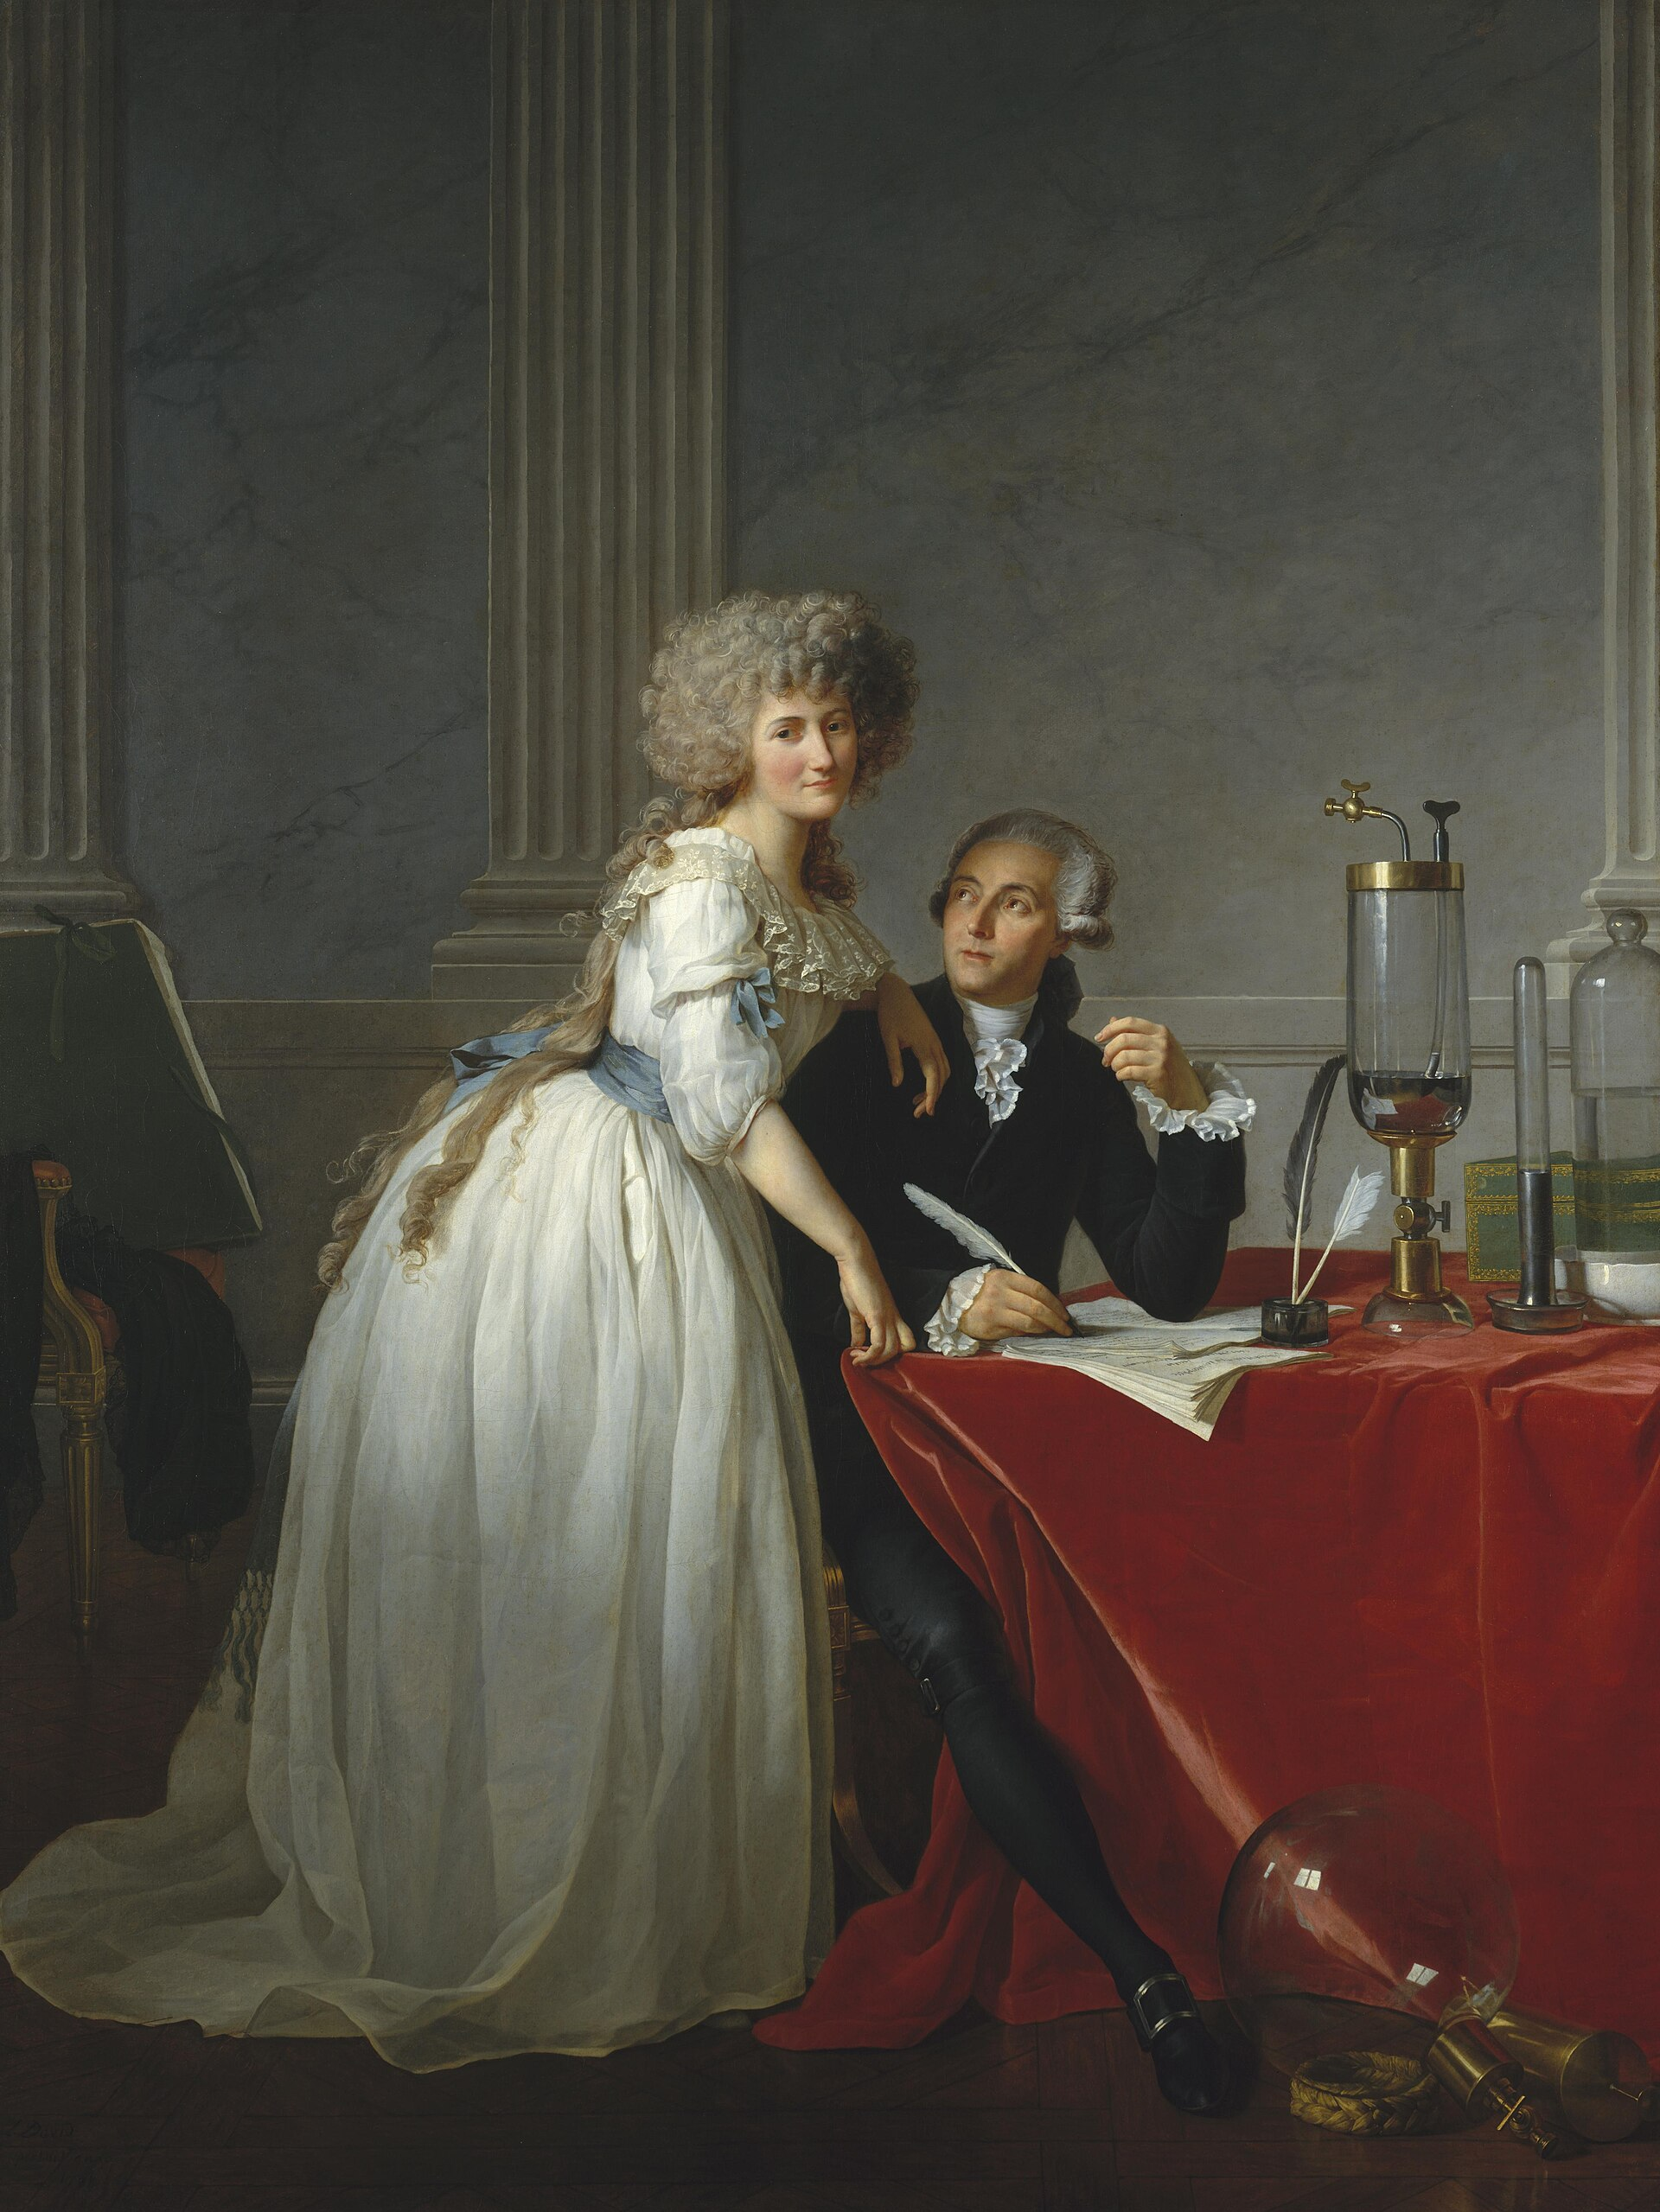
\includegraphics[width=0.3\linewidth]{images/book1/lavoisier.jpg}

{\small 安托万-洛朗·拉瓦锡与玛丽-安娜·保尔兹·拉瓦锡，
雅克-路易·大卫绘于 1788 年。}
\end{omfigure}

\section{质量为何守恒}

\begin{proposition}[原子守恒，因此质量守恒]\label{prop:g8:balanced-equations:why}
在反应中，\omterm{def:g7:atoms-and-molecules:atom}{原子}只是重新排列：\omterm{def:g7:chemical-reactions:reactant}{反应物}中的每一个\omterm{def:g7:atoms-and-molecules:atom}{原子}
都会在生成物中再次出现，每个\omterm{def:g7:atoms-and-molecules:atom}{原子}都保持自身的质量。
因此，总质量不可能改变。
\end{proposition}

\begin{example}[增重的铁]\label{ex:g8:balanced-equations:iron}
钢丝绒在敞口容器中放在天平上\omterm{def:g4:what-a-fire-needs:burning}{燃烧}，质量增加：铁
\omterm{def:g7:atoms-and-molecules:atom}{原子}与从\omterm{def:g4:air-a-mixture-of-gases:air}{空气}中夺取的氧\omterm{def:g7:atoms-and-molecules:atom}{原子}结合，生成的氧化铁
的质量等于铁加上这些氧的质量。若在装有\omterm{def:g4:air-a-mixture-of-gases:air}{空气}的密闭广口瓶中，
置于天平上\omterm{def:g4:what-a-fire-needs:burning}{燃烧}，则整体质量不变，
因为氧本来就在瓶内。
\end{example}

\section{化学方程式}

\begin{definition}[化学方程式]\label{def:g8:balanced-equations:equation}
\emph{化学方程式}\index{化学方程式}用化学式表示反应：
左边写出\omterm{def:g7:chemical-reactions:reactant}{反应物}的化学式，
各化学式之间用 $+$ 相连，中间加箭头，右边写出生成物的化学式。每个
化学式前面都可以加上一个数字。
若每种\omterm{def:g7:atoms-and-molecules:atom}{原子}在左右两边出现的次数都相同，则该方程式是
\emph{配平的方程式}\index{配平的方程式}。
\end{definition}

\begin{definition}[化学计量数]\label{def:g8:balanced-equations:coefficient}
方程式中写在化学式前面的数字，称为该化学式的
\emph{化学计量数}\index{化学计量数}：它
表示参与反应的该物质的\omterm{def:g7:atoms-and-molecules:molecule}{分子}（或其他粒子）数目。
化学计量数为 1 时不写出。
\end{definition}

\begin{notation}[状态符号]\label{not:g8:balanced-equations:states}
化学式后括号中的字母可以表示其物理状态：
(s) 固体，(l) 液体，(g) 气体。因此 \ce{H2O(l)} 表示液态水，
而 \ce{H2O(g)} 表示水蒸气。
\end{notation}

\begin{example}[读懂化学方程式]\label{ex:g8:balanced-equations:read}
\[
  \ce{CH4(g) + 2O2(g) -> CO2(g) + 2H2O(l)}
\]
读作：一个甲烷\omterm{def:g7:atoms-and-molecules:molecule}{分子}与两个氧气\omterm{def:g7:atoms-and-molecules:molecule}{分子}反应，生成一个
二氧化碳\omterm{def:g7:atoms-and-molecules:molecule}{分子}和两个水\omterm{def:g7:atoms-and-molecules:molecule}{分子}。左边：1 个 C，4 个 H，4 个 O。
右边：1 个 C，4 个 H，$2 + 2 = 4$ 个 O。该方程式已配平。
\end{example}

\begin{omfigure}
\begin{tikzpicture}[font=\small]
  \begin{scope}[every node/.style={font=\Large, inner sep=2pt}]
    \node (a) at (0,0) {\ce{CH4}};
    \node (p1) at (0.95,0) {$+$};
    \node (b) at (1.9,0) {\ce{2O2}};
    \node (arr) at (3.35,0) {$\longrightarrow$};
    \node (c) at (4.8,0) {\ce{CO2}};
    \node (p2) at (5.75,0) {$+$};
    \node (d) at (6.8,0) {\ce{2H2O}};
  \end{scope}
  \draw[thick, omDef] ([yshift=-2pt]a.south west) -- ++(0,-0.15) -| ([yshift=-2pt]b.south east);
  \node[below=8pt, text=black] at ($(a.south)!0.5!(b.south)$) {反应物};
  \draw[thick, omProp] ([yshift=-2pt]c.south west) -- ++(0,-0.15) -| ([yshift=-2pt]d.south east);
  \node[below=8pt, text=black] at ($(c.south)!0.5!(d.south)$) {生成物};
  \node[above=6pt of arr, font=\small] {“反应生成”};
  \node[anchor=north west, align=left, draw=black!35, rounded corners=2pt,
    font=\small, inner sep=4pt] at (-0.3,-1.25)
    {在 \ce{2O2} 中：前面的大号 2 是\textbf{化学计量数}（两个分子）；\\
     位于横线下方的小 2 是\textbf{下标}（每个分子含两个原子）。};
\end{tikzpicture}

{\small \omterm{def:g8:balanced-equations:equation}{化学方程式}的组成部分。}
\end{omfigure}

\section{配平化学方程式}

\begin{method}[配平化学方程式]\label{met:g8:balanced-equations:balance}
\begin{enumerate}
  \item 写出\omterm{def:g7:chemical-reactions:reactant}{反应物}和生成物的正确化学式。切记
        之后不可改动化学式：把 \ce{H2O} 改成 \ce{H2O2}，
        就成了描述另一种物质。
  \item 数一数两边每种\omterm{def:g7:atoms-and-molecules:atom}{原子}的个数。
  \item 每次只用\omterm{def:g8:balanced-equations:coefficient}{化学计量数}配平一种\omterm{def:g7:atoms-and-molecules:atom}{原子}，从
        两边各仅出现在一个化学式中的\omterm{def:g7:atoms-and-molecules:atom}{原子}开始；
        氢和氧最后再配。
  \item 再次数数，重复上述步骤，直至每种\omterm{def:g7:atoms-and-molecules:atom}{原子}都配平。
  \item \omterm{def:g8:balanced-equations:coefficient}{化学计量数}取最小的正整数。
\end{enumerate}
\end{method}

\begin{example}[氢和氧]\label{ex:g8:balanced-equations:water}
未配平：\ce{H2 + O2 -> H2O} % ce-unbalanced-ok (the skeleton)
左边有 2 个 O，右边有 1 个。在 \ce{H2O} 前加 2，此时右边有 4 个 H，
于是在 \ce{H2} 前加 2：
\[
  \ce{2H2 + O2 -> 2H2O}.
\]
检验：两边各有 4 个 H、2 个 O。
\end{example}

\begin{example}[铁在氧气中燃烧]\label{ex:g8:balanced-equations:iron-oxide}
铁与氧气反应生成氧化铁 \ce{Fe2O3}。氧：左边 2 个，
右边 3 个；最小公倍数为 6，故取 3 个 \ce{O2} 和 2 个
\ce{Fe2O3}。于是右边有 4 个 Fe，左边也取 4 个 Fe：
\[
  \ce{4Fe + 3O2 -> 2Fe2O3}.
\]
\end{example}

\begin{omfigure}
\begin{tikzpicture}[font=\small]
  % 2 H2
  \foreach \y in {0.45,-0.45} {
    \node[aH] (a) at (0,\y) {}; \node[aH] (b) at (0.45,\y) {};
    \begin{scope}[on background layer]\draw[bond] (a.center) -- (b.center);\end{scope}}
  \node at (1.05,0) {$+$};
  \node[aO] (a) at (1.6,0) {}; \node[aO] (b) at (2.25,0) {};
  \begin{scope}[on background layer]
    \draw[bond, line width=1.1pt] ([yshift=1.6pt]a.center) -- ([yshift=1.6pt]b.center);
    \draw[bond, line width=1.1pt] ([yshift=-1.6pt]a.center) -- ([yshift=-1.6pt]b.center);
  \end{scope}
  \draw[->, thick, omProp] (2.9,0) -- (3.9,0);
  \foreach \y in {0.5,-0.5} {
    \node[aO] (o) at (4.9,\y+0.12) {};
    \node[aH] (p) at (4.35,\y-0.28) {}; \node[aH] (q) at (5.45,\y-0.28) {};
    \begin{scope}[on background layer]
      \draw[bond] (o.center) -- (p.center); \draw[bond] (o.center) -- (q.center);
    \end{scope}}
  \node[align=center, font=\footnotesize] at (1.1,-1.35) {4 个 H，2 个 O};
  \node[align=center, font=\footnotesize] at (4.9,-1.35) {4 个 H，2 个 O};
  \node[font=\small] at (2.7,-2.0) {\ce{2H2 + O2 -> 2H2O}};
\end{tikzpicture}

{\small 氢气\omterm{def:g4:what-a-fire-needs:burning}{燃烧}的配平方程式，用模型图表示：
两个氢气\omterm{def:g7:atoms-and-molecules:molecule}{分子}与一个氧气\omterm{def:g7:atoms-and-molecules:molecule}{分子}反应，生成两个水
\omterm{def:g7:atoms-and-molecules:molecule}{分子}。}
\end{omfigure}

\section{从分子角度读化学方程式}


\begin{proposition}[配平的方程式表示什么]\label{prop:g8:balanced-equations:molecules}
\omterm{def:g8:balanced-equations:equation}{配平的方程式}中的\omterm{def:g8:balanced-equations:coefficient}{化学计量数}，给出粒子
参加反应和生成的比例关系。若方程式写为
\ce{2H2 + O2 -> 2H2O}，则 200 个氢气\omterm{def:g7:atoms-and-molecules:molecule}{分子}与 100 个
氧气\omterm{def:g7:atoms-and-molecules:molecule}{分子}反应，生成 200 个水\omterm{def:g7:atoms-and-molecules:molecule}{分子}；一百万个氧气\omterm{def:g7:atoms-and-molecules:molecule}{分子}
需要两百万个氢气\omterm{def:g7:atoms-and-molecules:molecule}{分子}。
\end{proposition}

\begin{example}[露营炉中的丙烷]\label{ex:g8:balanced-equations:propane}
丙烷 \ce{C3H8} 在氧气中\omterm{def:g4:what-a-fire-needs:burning}{燃烧}，生成二氧化碳和水。
先配碳：3 个 C，故写 3 \ce{CO2}。氢：8 个 H，故写 4 \ce{H2O}。配氧，
右边共 $3 \times 2 + 4 = 10$ 个 O，故写 5 \ce{O2}：
\[
  \ce{C3H8 + 5O2 -> 3CO2 + 4H2O}.
\]
每个丙烷\omterm{def:g7:atoms-and-molecules:molecule}{分子}需要 5 个氧气\omterm{def:g7:atoms-and-molecules:molecule}{分子}。
\end{example}

\section{练习}

\begin{exercise}[$\star$]\label{exo:g8:balanced-equations:1}
陈述\omterm{def:g8:balanced-equations:conservation}{质量守恒}定律。
\end{exercise}

\begin{exercise}[$\star$]\label{exo:g8:balanced-equations:2}
在 \ce{3CO2} 中，\omterm{def:g8:balanced-equations:coefficient}{化学计量数}是多少？它表示多少个碳
\omterm{def:g7:atoms-and-molecules:atom}{原子}和多少个氧\omterm{def:g7:atoms-and-molecules:atom}{原子}？
\end{exercise}

\begin{exercise}[$\star$]\label{exo:g8:balanced-equations:3}
\ce{C + O2 -> CO2} 是否已配平？数一数\omterm{def:g7:atoms-and-molecules:atom}{原子}个数以检验。
\end{exercise}

\begin{exercise}[$\star$]\label{exo:g8:balanced-equations:4}
配平 \ce{Mg + O2 -> MgO}。 % ce-unbalanced-ok (to balance)
\end{exercise}

\begin{exercise}[$\star\star$]\label{exo:g8:balanced-equations:5}
配平 \ce{N2 + H2 -> NH3}，这是合成氨的反应。 % ce-unbalanced-ok (to balance)
\end{exercise}

\begin{exercise}[$\star\star$]\label{exo:g8:balanced-equations:6}
\qty{12}{g} 的碳完全\omterm{def:g4:what-a-fire-needs:burning}{燃烧}，生成 \qty{44}{g} 的
二氧化碳。消耗氧气的质量是多少？
\end{exercise}

\begin{exercise}[$\star\star$]\label{exo:g8:balanced-equations:7}
观察图中天平上的两个烧瓶。为什么敞口烧瓶的
读数会下降？质量被消灭了吗？
\end{exercise}

\begin{exercise}[$\star\star$]\label{exo:g8:balanced-equations:8}
逐步配平 \ce{CH4 + O2 -> CO2 + H2O}，并说明每一步 % ce-unbalanced-ok (to balance)
配平的是哪一种\omterm{def:g7:atoms-and-molecules:atom}{原子}。
\end{exercise}

\begin{exercise}[$\star\star$]\label{exo:g8:balanced-equations:9}
某同学想配平 \ce{H2 + O2 -> H2O}，他把它写成 \ce{H2 + O2 -> H2O2}。 % ce-unbalanced-ok (the student's start)
为什么这样做是错误的？
\end{exercise}

\begin{exercise}[$\star\star$]\label{exo:g8:balanced-equations:10}
利用 \ce{C3H8 + 5O2 -> 3CO2 + 4H2O}，\omterm{def:g4:what-a-fire-needs:burning}{燃烧} 20 个丙烷\omterm{def:g7:atoms-and-molecules:molecule}{分子}
需要多少个氧气\omterm{def:g7:atoms-and-molecules:molecule}{分子}？能生成多少个
水\omterm{def:g7:atoms-and-molecules:molecule}{分子}？
\end{exercise}

\begin{exercise}[$\star\star\star$]\label{exo:g8:balanced-equations:11}
配平 \ce{C2H6 + O2 -> CO2 + H2O}，这是乙烷的\omterm{def:g4:what-a-fire-needs:burning}{燃烧}。（提示：试着 % ce-unbalanced-ok (to balance)
把乙烷的\omterm{def:g8:balanced-equations:coefficient}{化学计量数}加倍。）
\end{exercise}

\begin{exercise}[$\star\star\star$]\label{exo:g8:balanced-equations:12}
一支 \qty{20.0}{g} 的蜡烛在充满\omterm{def:g4:air-a-mixture-of-gases:air}{空气}的密闭玻璃箱中\omterm{def:g4:what-a-fire-needs:burning}{燃烧}，该箱
放在天平上，天平读数共为 \qty{850.0}{g}。火焰熄灭时，
蜡烛的质量为 \qty{19.6}{g}。此时天平的读数是多少？请说明理由。
\end{exercise}

\section{问题：密闭广口瓶中的钢丝绒}

\begin{problem}[{周末问题——能燃烧的铁，示数不变的天平，
以及取自空气的氧气}]
\label{pb:g8:balanced-equations:1}
在实验室中，老师\omterm{def:g4:what-a-fire-needs:burning}{燃烧}钢丝绒，它几乎是纯铁，
分两种方式进行。第一种，将一团钢丝绒放在天平上的敞口培养皿中\omterm{def:g4:what-a-fire-needs:burning}{燃烧}，
示数增大。然后，取质量为 \qty{0.28}{g} 的一团钢丝绒，
用电火花点燃，放在天平上密闭的\omterm{def:g4:air-a-mixture-of-gases:air}{空气}广口瓶中：示数
不变。该广口瓶中约含 \qty{0.5}{g} 氧气。
铁在氧气中\omterm{def:g4:what-a-fire-needs:burning}{燃烧}生成氧化铁 \ce{Fe2O3}；氧气不足时，
还可生成 \ce{Fe3O4}。

\medskip
\noindent\textbf{第一部分——两次称量。}
\begin{enumerate}
  \item 敞口培养皿中的质量增大了。多出的质量
        来自何处？
  \item 在密闭广口瓶中，质量不变。请解释原因。
  \item 陈述这两次称量所说明的定律。
\end{enumerate}

\medskip
\noindent\textbf{第二部分——两个\omterm{def:g8:balanced-equations:equation}{化学方程式}。}
\begin{enumerate}[resume]
  \item 配平方程式 \ce{Fe + O2 -> Fe2O3}。 % ce-unbalanced-ok (to balance)
  \item 配平方程式 \ce{Fe + O2 -> Fe3O4}。 % ce-unbalanced-ok (to balance)
  \item 通过数第一个方程式两边
        每种\omterm{def:g7:atoms-and-molecules:atom}{原子}的个数来检验。
  \item 根据第一个方程式，
        与 400 个铁\omterm{def:g7:atoms-and-molecules:atom}{原子}反应的氧气\omterm{def:g7:atoms-and-molecules:molecule}{分子}有多少个？
\end{enumerate}

\medskip
\noindent\textbf{第三部分——质量。}
在 \ce{Fe2O3} 中，每 \qty{7}{g} 铁与 \qty{3}{g} 的
氧气化合。这团 \qty{0.28}{g} 的钢丝绒完全\omterm{def:g4:what-a-fire-needs:burning}{燃烧}生成 \ce{Fe2O3}。
\begin{enumerate}[resume]
  \item 与 \qty{0.28}{g} 铁化合的氧气质量是多少？
  \item 生成的氧化铁质量是多少？
  \item 广口瓶中的氧气是否足够？请说明理由。
  \item 冷却后打开广口瓶，\omterm{def:g4:air-a-mixture-of-gases:air}{空气}涌入。请解释原因，
        并说明此时天平的读数如何变化。
  \item 计算钢丝绒\omterm{def:g4:what-a-fire-needs:burning}{燃烧}时取自广口瓶
        中\omterm{def:g4:air-a-mixture-of-gases:air}{空气}的氧气质量。
\end{enumerate}
\end{problem}
